\documentclass{article}

\htmlpath{../../qadil/htmlinclude/}
\includehtml{metainfo}
\includehtml{jquery3.1.0}
\includehtml{katex0.12.0}
\includehtml{bootstrap3.3.7}
\includehtml{index}
\includehtml{sidebar}
 
\title{Example of notes}
\author{Niels Lauritzen}

\begin{document}[sidebar]

\maketitle

\vspace{2cm}

\begin{changemargin}{3cm}{3cm}
  Here is an example abstract! Below you should see inclusion of
  an image file. The burger in the upper left hand corner is the entry
  to the clickable table of contents. The first and only chapter in the generic notes is the \emph{Language of mathematics} chapter from  the \url{IMO course}{https://edtech.dk/IMO} given in the fall of 2020.
\end{changemargin}



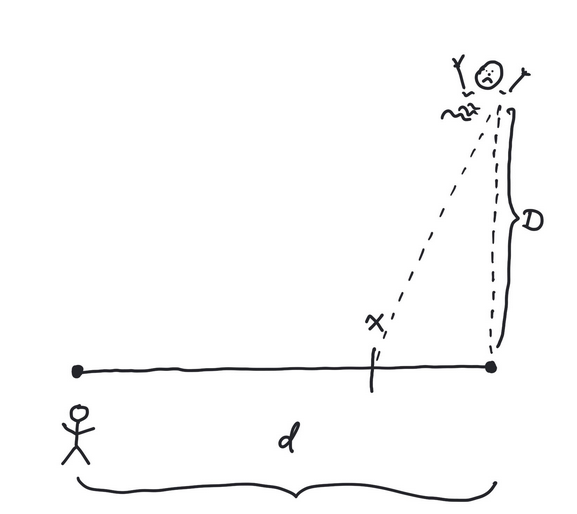
\includegraphics{lifeguard.png}


\end{document}











